\documentclass[a4paper,12pt]{article}
\usepackage{amsmath,amssymb,amsfonts,amsthm}
\usepackage{tikz}
\usepackage[utf8x]{inputenc}
\usepackage[T2A]{fontenc} 
\usepackage[russian]{babel}
\usepackage{cmap} 
\usepackage{ gensymb }
% Так ссылки в PDF будут активны
\usepackage[unicode]{hyperref}
\usepackage{ textcomp }
\usepackage{indentfirst}
\usepackage[version=3]{mhchem}

% вы сможете вставлять картинки командой \includegraphics[width=0.7\textwidth]{ИМЯ ФАЙЛА}
% получается подключать, как минимум, файлы .pdf, .jpg, .png.
\usepackage{graphicx}
\usepackage{wrapfig}
% Если вы хотите явно указать поля:
\usepackage[margin=1in]{geometry}
% Или если вы хотите задать поля менее явно (чем больше DIV, тем больше места под текст):
% \usepackage[DIV=10]{typearea}

\usepackage{fancyhdr}

\newcommand{\bbR}{\mathbb R}%теперь вместо длинной команды \mathbb R (множество вещественных чисел) можно писать короткую запись \bbR. Вместо \bbR вы можете вписать любую строчку букв, которая начинается с '\'.
\newcommand{\eps}{\varepsilon}
\newcommand{\bbN}{\mathbb N}
\newcommand{\dif}{\mathrm{d}}

\newtheorem{Def}{Определение}


\pagestyle{fancy}
\makeatletter % сделать "@" "буквой", а не "спецсимволом" - можно использовать "служебные" команды, содержащие @ в названии
\fancyhead[L]{\footnotesize Лабораторные работы по общей физике}%Это будет написано вверху страницы слева
\fancyhead[R]{\footnotesize ФУПМ МФТИ}
%\fancyfoot[L]{\footnotesize \@author}%имя автора будет написано внизу страницы слева
\fancyfoot[R]{\thepage}%номер страницы —- внизу справа
\fancyfoot[C]{}%по центру внизу страницы пусто

\renewcommand{\maketitle}{%
	\noindent{\bfseries\scshape\large\@title\ \mdseries\upshape}\par
	\noindent {\large\itshape\@author}
	\vskip 2ex}
\makeatother
\def\dd#1#2{\frac{\partial#1}{\partial#2}}


\title{2.2. Измерение длин волн спектральных линий водорода}
\author{Хурсик Екатерина} 
\date{\today}

\begin{document}
	
\maketitle
\section{Цель работы}
Исследовать спектральные закономерности в оптическом спектре водорода.
По результатам измерений вычислить постоянные Ридберга.

 
\section{Ход работы}
\subsection*{Калибровка спектрометра}
$$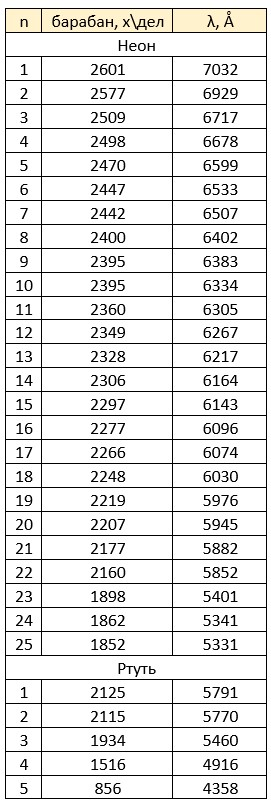
\includegraphics[width=0.35\linewidth]{2020-10-07-2.jpg}$$
$$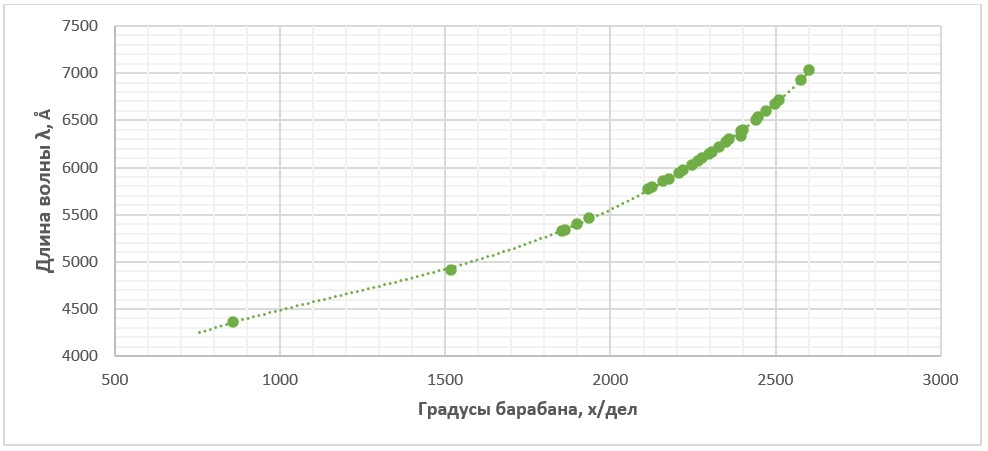
\includegraphics[width=1.1\linewidth, height=0.3\textheight]{2020-10-07-3.jpg}$$
\subsection*{Определение длин волн спектра водорода}
Измерим положение линий $H_\alpha$, $H_\beta$, $H_\gamma$ (линия $H_\delta$ не видна)
и с помощью калибровочного графика определим их длины волн. Результаты сведём
в таблицу 
 
\begin{table}[h!]
    \begin{center}
        \begin{tabular}{|c|c|c|c|c|c|c|c|c|}
            \hline 
            Линия спектра & $ \theta $, $ ^\circ $ & $ \lambda, \;\mathring{A} $ & $ m $  & $ \frac{1}{\lambda}, \;  10^{-4} \mathring{A}^{-1}\text{(рассч.)} $  & $\varepsilon,\,\%$ & $ \sigma(\frac{1}{\lambda}), 10^{-4} \mathring{A}^{-1} $ & $ \frac{1}{\lambda}, \;  10^{-4} \mathring{A}^{-1} $\\ 
            \hline 
        $ H_\alpha $ & 2452 & 6578 & 3  & 1.524 & 0.8 & 0.012 & $1.520\pm0.012$\\
        $ H_\beta $  & 1464 & 4901 & 4  & 2.058 & 1 & 0.021 & $2.040\pm0.021$\\
        $ H_\gamma $ & 838 & 4333 & 5  & 2.304 & 1.2 & 0.028 & $2.308\pm0.028$\\
            \hline 
        \end{tabular} 
    \end{center}
    \caption{Определение линий спектра водорода}
    \label{table_mn}
\end{table}

Исходя из определённых нами длин волн (с учётом погрешностей) по калибровочному графику убеждаемся,
что отношение длин волн водородных линий соответствует отношениям длин волн, вычисленных по формуле (1).

Для каждой из наблюдаемых линий водорода вычислим значение постоянной Ридберга
\begin{equation*}
    R_{H}=\frac{1}{\lambda(\frac{1}{n^2}-\frac{1}{m^2})}\,\rightarrow\, R_{H_\alpha}=109455,8\, \text{см}^{-1},\, R_{H_\beta}=108821,3 \,\text{см}^{-1},\, R_{H_\gamma}=109898,6 \,\text{см}^{-1}
\end{equation*}
Определим среднее значение постоянной Ридберга по всем измерениям:
\begin{equation*}
    <R_H>=\frac{R_{H_\alpha}+R_{H_\beta}+R_{H_\gamma}}{3}=109391,8\,\text{см}^{-1}
\end{equation*}
Определим погрешность измерения постоянной Ридберга $\sigma(R_H)$:
\begin{equation*}
    \sigma(R_H)=\sqrt{\frac{1}{n(n-1)}\sum\limits_{i=1}^n(R_{H_i}-<R_H>)^2}=\sqrt{\frac{1}{3\cdot2}\sum\limits_{i=1}^n(R_{H_i}-<R_H>)^2}=312,6 \,\text{см}^{-1}, \varepsilon_\sigma=0,3\%
\end{equation*}
\begin{equation*}
    \varepsilon_{R_H}=\sqrt{\varepsilon_{\sigma}^2+\varepsilon_{R_{H_\alpha}}^2+\varepsilon_{R_{H_\beta}}^2+\varepsilon_{R_{H_\gamma}}^2}=2,1 \%
\end{equation*}
Получаем постоянную Ридберга равную
\begin{equation*}
    R_H=109391,8\pm2297,3\, \text{см}^{-1}, \,\varepsilon = 2,1\%
\end{equation*}
Сравнивая полученное значение постоянной Ридберга с рассчётным $R_H=109677,6 \,\text{см}^{-1}$,
заключаем, что получили совпадающее в пределах погрешности значение.
\section{Вывод}
1) Измерили положения линий $H_\alpha$, $H_\beta$, $H_\gamma$ (линия $H_\delta$ не видна). Построили градуировочный график, подобрав для градуировочной кривой кубический сплайн.
Кривая при этом легла достаточно точно на измеренные точки.

2) Убедились в том, что полученные отношения длин волн водородных линий
соответствуют обобщённой формуле Бальмера.

3) Нашли постоянную Ридберга, которая в пределах погрешности совпадает с табличной.


    
\end{document}
